\section{\compiler\ Implementation}
Given the map algebra shown in the previous section, we now describe
the implementation of \compiler, including a couple of data structures it
uses, and two extensions considering adaptive query execution based on runtime
trends.

\subsection{\compiler\ Data Structures}
The key data structure in\\\compiler\ is an
associative map.
While this map can
always be implemented in a straightforward manner by a hashtable, its usage is
primarily governed by the map algebra expression directly using involving the
bound variable (i.e. the map key). In this section we consider bound
variable use in predicate expressions, namely in a range predicate and a window
predicate, which are effectively one- and two-sided ranges, motivating the use
of interval data structures. In general, the choice of data structure used as a
map for an arbitrary map algebra expression is an open question, and the work
here primarily considers conjunctive equality or range predicates.

\textbf{Range predicates.}
In the case of a range predicate, a bound variable $x$ is used as part of an
aggregate query over tuples filtered by $x$. Hence increasing values of $x$
result in a larger aggregation set, and in the case of the \texttt{sum} and
\texttt{max} aggregates, a map binding that can be computed from neighboring
values to $x$. Thus the data structure is effectively a cumulative data
structure, where each $x$ maintains the result of an aggregation function between
query attributes limited by $x$ and the aggregate value compute for a neighbor
$x^-$ (or $x^+$ depending on the comparison operator in the predicate). This can
be implemented by a binary tree data structure for accessing neighbor keys, as
opposed to a hashtable. Note that the variable $x$ can be bound to values in an
arbitrary order, requiring the ability to insert and delete bindings at any point
within the data structure. While the binary tree suffices for our purposes here,
deriving an optimal data structure with these characteristics is a topic for
future work.

\textbf{Window predicates.}
In contrast to range predicates, window predicates are two-sided and apply to
non-decreasing values of variable bindings for $x$. With such properties in the
addition and removal of variable bindings, a doubly linked list data structure
sorted on binding value turns out to be extremely efficient for handling the map. Note
that lookups also have a specific property here, it is always the largest bound
value that is accessed, hence by providing constant time lookup, insertion and
removal at both ends, a doubly linked list is optimal.

\begin{figure}[htbp]
\begin{center}
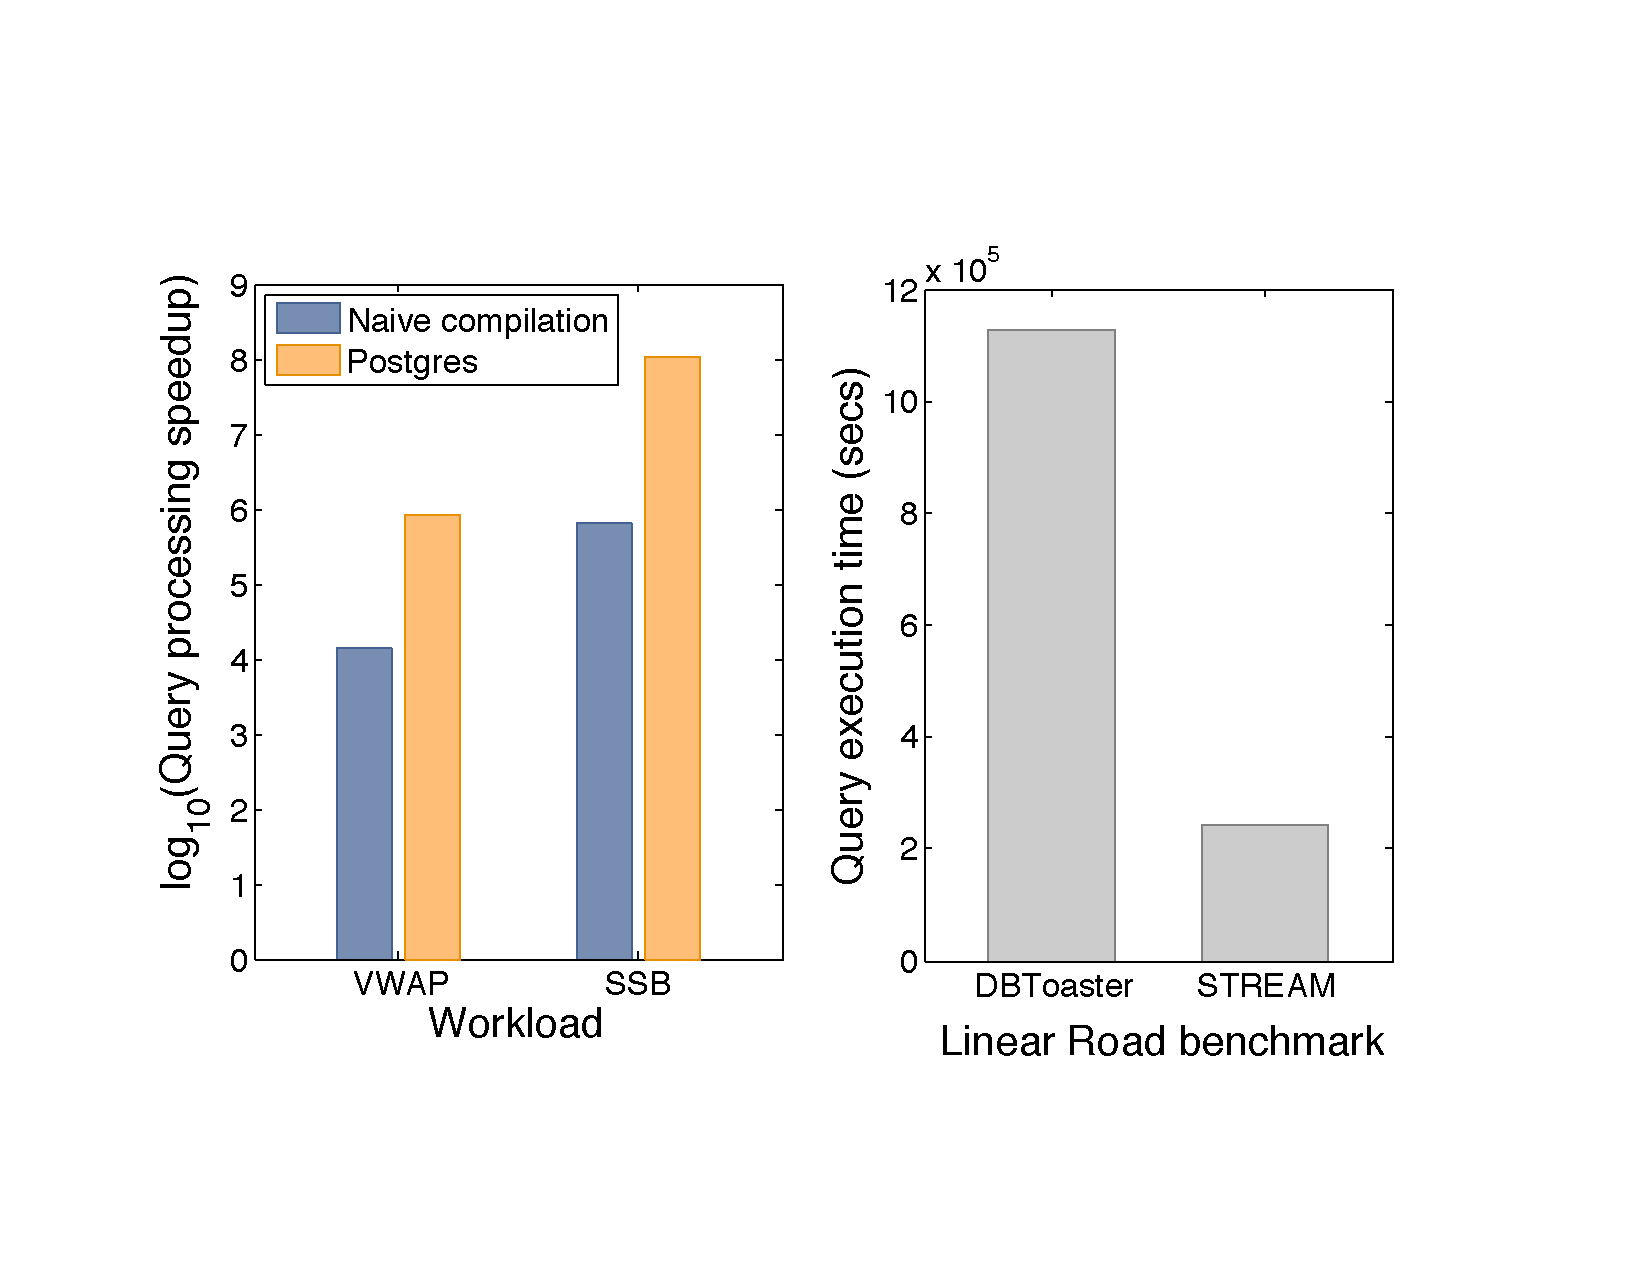
\includegraphics[scale=0.4]{../plots/toaster_comparison.pdf}
\end{center}
\vspace{-4mm}
\caption{Query processing performance comparison of compiled query executors
generated by DBToaster and plan compilation, Postgres and STREAM}
\label{fig:dbtperf}
\end{figure}


\subsection{Adaptive Query Executors}

To this point, we have described a compiler to produce static main-memory query
executor, which incorporates both standard rewrite rules for query optimization
and our custom rules for compilation. The choice of optimal query plans is
subject to the contents of the input relations being processed, leading to the
challenges of query reoptimization and adaptive query processing. In this section
we consider extensions to provide adaptive query execution in our generated code.
For \compiler, this involves producing several plans and generating the
monitoring and decision-making logic to determine which plan to evaluate based on
statistics collected at runtime. We present this section as a discussion of the
relevance and impact of key adaptation techniques in our context, rather than a
focusing on detailed algorithms that reshape such techniques to apply in
\compiler.

\comment{
\subsection{Memory Usage Analysis}
\begin{itemize}
  \item Apply to generalized join graphs, and their hypertree decomposition.
  \item Given a tree-structured join graph, analyse map construction rules and
  discuss based on fanout of nodes in the join graph.
  \item The analysis approach should be to generalize each rewrite rule, compute
  the incremental space usage from each rewrite rule, and finally reason about
  the size of the decomposition tree. The size of this decomposition tree can
  be derived from the hypertree structure.
  \item Consider our standard example template:\linebreak
  $sum(a_1, \ldots , a_n) R,S,T_1,\ldots T_{n-1}$, where there is a $n-way$ join.
  This is a simple join tree of height 2 with $n$ leaves and a single root. Our
  decomposition tree has width $n - level$ at each level and height $n$. The
  number of maps is thus bounded by $\sum_{i=0}^{n-1}{(i+1)*(n-i)} =
  \sum_{i=1}^{n}{(n+1-i)*i} = (n+1)\sum_{i=1}^{n}{i} - \sum_{i=1}^{n}{i^2}$
  \linebreak $= \frac{(n+1)n(n-1)}{2} - \frac{2n^3-3n^2+n}{6} = O(n^3)$.
  Note this includes many duplicate maps, which we'll need to quantify to get a
  tighter bound ($O(n^3)$ is sizeable, even if $n$ is usually small given it's
  the number of relations). Furthermore this does not say anything about the size
  of each map, which we'll have to reason about in terms of the domain sizes for
  each attribute.
  
  \item Assume each leaf in the join tree contributes an aggregation column and
  potentially group-by columns. Internal nodes may or may not contribute
  aggregation columns and group by columns. Internal nodes consist of at least
  one join predicate column.
\end{itemize}
}

\textbf{Batch processing.} 
Simple update or query batching is a common technique used in a variety of query
processors to take advantage of machine-level characteristics in modern computer
architectures, including pipelining, various levels of caches, as well as
vectorized instructions. In addition to these benefits which apply under the hood
of the native code generated, we consider the effects of unrolling the main delta
loop on update batches, creating a table of batch processing functions each
capable of supporting different length batches. While this results in a larger
code size, SQL queries tend to be relatively small and our generated binaries are
on the order of kilobytes or megabytes, and thus code size ifs not a concern at
this stage. We invoke batch processing functions through a signature matching
scheme, where a batch function's signature is simply a specific sequence of data
manipulations (e.g. 4 inserts). For simplicity, and efficient batch detection, we
consider simple patterns as signatures, restricting ourselves to $k$-length
sequences of a single type of data manipulation (i.e. $k$-inserts or $k$-deletes)
for a fixed range of $k$ values.

While more complex batch and pattern detection has been applied, for example for
prefetching as in Scalpel~\cite{bowman-tods:05}, we make the following
observation. As we will see in the experimental evaluation, we produce a highly
efficient executor as the result of our compilation, implying we require a
commensurate improvement in the monitoring conditions that determine when to
adapt running plans. However, these monitoring conditions are typically
implemented by database developers directly in the engine, and are already
operating with low overhead. This entails our design principle that only simple
and extremely lightweight adaptations are of use in a compiled query executor due
to the increasing cost of monitoring relative to processing.

\comment{
\begin{itemize}
  \item Improve pipelining by unrolling the main delta loop, and
  applying independent lines of code in sequence. We refer to applying
  $k$ independent statements in sequence as $k$-level unrolling.
  \item We consider more structured sequences, i.e. patterns perhaps from
  a profiling process based on frequent pattern mining on the delta workload,
  and apply dead-code elimination based on the pattern.
  \item We may want to exploit vectorized instructions, e.g. Altivec/SSE
  instructions. We probably won't go into much depth on this due to limited
  research impact. Generally the goal in this paper is not to build a
  high-performance backend that will take C code and produce tight
  instruction-level code. We leave room for this given our choice of using
  the LLVM framework which will allow modular development of our compilation
  toolchain, but will revisit low-level implementation issues in the future.
  \item Challenge: statically picking the right chunk size for processing, given
  profiling information. We can't handle changes in delta rates to different base
  relations (e.g., no adaptive unrolling/pipelining). How much does this kill the
  argument?
  \item What are the caching effects of bulk operations? Bulk operations should
  improve cache hit ratios as long as the portions of the data structures used
  fit in cache (as working sets). We may want to pick the right chunk size at the
  limit of beneficial pipelining and caching effects, i.e. when one of these two
  advantages starts to become a drawback.
\end{itemize}
}


\textbf{Lazy map maintenance.}
\compiler\ considers evaluating its tuple functions eagerly or lazily, resulting
in a deferred approach to maintaining map structures for producing results given
inputs to other relations. By default, \compiler\ adopts an eager evaluation
strategy, updating map structures for all other parts of the query, given a
single input tuple. Lazy map maintenance is advantageous in scenarios where there
is at least one significantly lagging input, resulting in uncessary eager updates
of the remaining map structures. Taking advantage of the opportunity to be lazy
requires two additional pieces of generated code. The first of these is a simple
profiler that captures update rate statistics to determine candidates for lazy
evaluation. Based on a cost model of these statistics, the second piece of
generated code is a conditional where on one branch, the executor enqueues the
delta to local state associated with the map structure at the point of deferral.
Note we can apply simplifications of those deltas in local state, which may
cancel each other out, or may be merged into a single delta. The tuple function
returns control to the event loop at this point, ready to process the next
available delta.


\comment{  
\textbf{Limitations.}
\begin{itemize}
  \item We profile delta rates on each base relation, and compute internal
  selectivities to determine when to defer updating a map while processing a
  kernel function.
  \item In terms of code generation this adds conditionals based on profiling
  statistics around each map update, where one branch updates the map as before,
  and the other branch stores the delta to be applied at some later point. Note
  given the recursive nature of our decomposition, we jump out of the kernel
  function and handle the next delta on the first branch indicating deferral.
  \item How do we store the deferred updates? As queues associated with each
  map?
  \item This may cause a large number of long jumps in our code, how will this
  affect performance, e.g. what are the effects on branch prediction, I-cache
  performance, etc.?
\end{itemize}
}

\comment{
\subsection{Multi-query compilation and map sharing}
Given that each query is decomposed into a set of map structures, queries
operating on similar sets of input relations are likely to be able to share
such structures in a similar fashion to multi-query optimization. 
}

\comment{
\subsection{Discussion: adaptivity limitations}

\begin{itemize}
  \item Compilation and adaptivity are inherently in tension, pulling engines
  in opposite directions.
  \item TODO: how can we show we are not going to do too badly regardless of how
  the delta workload changes? Perhaps we can borrow ideas from robust query
  processing, where they pick a plan based on maximizing the parameter space
  (i.e. of those statistics profiled) covered by a single plan, as the choice of
  plan we decompose.
\end{itemize}
}
